\section{Representación del ejercicio 2}
Se utilizó un ciclo \textbf{para} con 20 repeticiones. En cada mes se mostró el pago, se sumó al total y se duplicó para la siguiente iteración. El pago mensual siguió $p_m=10\cdot2^{m-1}$.
\begin{singlespace}
\noindent\begin{minipage}[t]{.43\linewidth}
\textbf{Pseudocódigo}
\begin{lstlisting}
pago <- 10
total <- 0
Para mes <- 1 hasta 20
  Mostrar mes, pago
  total <- total + pago
  pago <- pago * 2
FinPara
Mostrar total
\end{lstlisting}
\end{minipage}\hfill
\begin{minipage}[t]{.54\linewidth}
\centering\textbf{Diagrama de flujo}\\[4pt]
\begin{tikzpicture}[
  font=\footnotesize,
  e2terminal/.style={draw,rounded corners,minimum width=1.4cm,
    minimum height=.5cm,align=center,inner sep=3pt},
  e2proceso/.style={draw,rectangle,text width=2.9cm,
    minimum height=.65cm,align=center,inner sep=4pt},
  e2decision/.style={draw,diamond,aspect=2,text width=1.5cm,
    align=center,inner sep=2pt},
  e2entrada/.style={draw,trapezium,trapezium left angle=75,
    trapezium right angle=105,text width=2cm,
    align=center,inner sep=4pt},
  e2flecha/.style={-{Stealth[length=2mm]}}
]
\node[e2terminal] (ini) {Inicio};
\node[e2proceso,below=4mm of ini] (init)
  {$pago\gets10$\\$total\gets0$\\$mes\gets1$};
\node[e2decision,below=5mm of init] (ciclo) {$mes\leq20$};
\node[e2entrada,below=6mm of ciclo] (mostrar)
  {Mostrar\\mes y pago};
\node[e2proceso,below=4mm of mostrar] (sum)
  {$total\gets total+pago$};
\node[e2proceso,below=4mm of sum] (dup)
  {$pago\gets pago\cdot2$\\$mes\gets mes+1$};
\node[e2entrada,text width=1.3cm,right=8mm of ciclo,yshift=-1.5cm]
  (sal) {Mostrar\\total};
\node[e2terminal,below=4mm of sal] (fin) {Fin};
\draw[e2flecha] (ini.south)--(init.north);
\draw[e2flecha] (init.south)--(ciclo.north);
\draw[e2flecha] (ciclo.south)--node[right]{Sí}(mostrar.north);
\draw[e2flecha] (mostrar.south)--(sum.north);
\draw[e2flecha] (sum.south)--(dup.north);
\draw[e2flecha] (ciclo.east)-|node[above,pos=.25]{No}(sal.north);
\draw[e2flecha] (sal.south)--(fin.north);
\draw[e2flecha] (dup.south)--++(0,-4mm)--++(-2.4cm,0)
  |- (ciclo.west);
\end{tikzpicture}
\end{minipage}
\par\vspace{1cm}
\noindent\textbf{Diagrama N/S}
\begin{center}
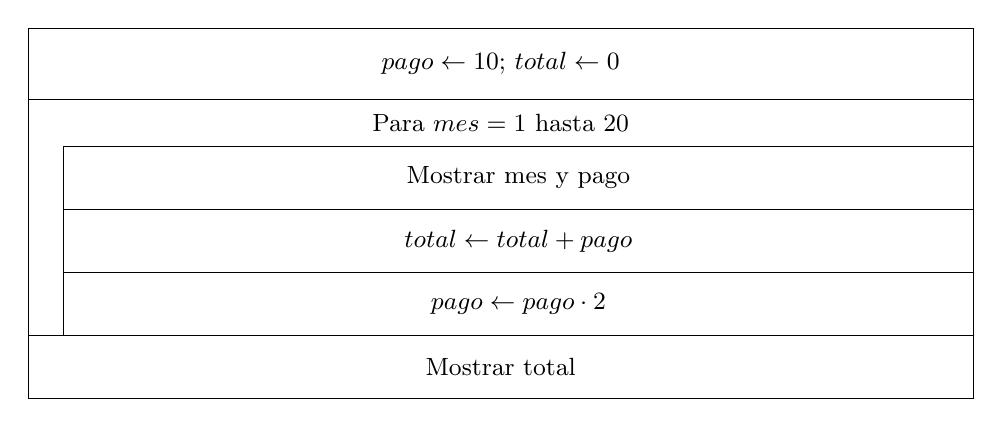
\begin{tikzpicture}[x=1cm,y=1cm,font=\small]
% Cabecera horizontal del ciclo para evitar texto vertical superpuesto.
\draw (0,0) rectangle (12,4.7);
\draw (0,3.8)--(12,3.8);
\node at (6,4.25) {$pago\gets10$; $total\gets0$};
\node at (6,3.5) {Para $mes=1$ hasta $20$};
\draw (.45,3.2)--(12,3.2);
\draw (.45,.8)--(.45,3.2);
\draw (.45,2.4)--(12,2.4);
\draw (.45,1.6)--(12,1.6);
\node at (6.225,2.8) {Mostrar mes y pago};
\node at (6.225,2) {$total\gets total+pago$};
\node at (6.225,1.2) {$pago\gets pago\cdot2$};
\draw (0,.8)--(12,.8);
\node at (6,.4) {Mostrar total};
\end{tikzpicture}
\end{center}
\end{singlespace}
